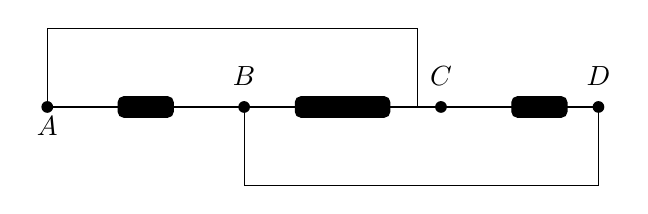
\begin{tikzpicture}[x=1cm,y=1cm]
  % main horizontal wire with nodes A,B,C,D
  \draw (0,0) -- (7,0);
  \node[circle,fill,inner sep=1.5pt] at (0,0) {};
  \node[circle,fill,inner sep=1.5pt] at (2.5,0) {};
  \node[circle,fill,inner sep=1.5pt] at (5,0) {};
  \node[circle,fill,inner sep=1.5pt] at (7,0) {};
  \node[below] at (0,0) {$A$};
  \node[above] at (2.5,0.15) {$B$};
  \node[above] at (5,0.15) {$C$};
  \node[above] at (7,0.15) {$D$};
  % resistor blocks (filled rounded rectangles) between A-B, B-C, C-D
  \draw[fill=black,rounded corners=2pt] (0.9,-0.13) rectangle (1.6,0.13);
  \draw[fill=black,rounded corners=2pt] (3.15,-0.13) rectangle (4.35,0.13);
  \draw[fill=black,rounded corners=2pt] (5.9,-0.13) rectangle (6.6,0.13);
  % top jumper wire: from A, up and over, down to just before C
  \draw (0,0) -- (0,1) -- (4.7,1) -- (4.7,0);
  % bottom jumper wire: from B, down and over, up to D
  \draw (2.5,0) -- (2.5,-1) -- (7,-1) -- (7,0);
\end{tikzpicture}
